\documentclass[a4paper, 11pt]{article} % Uses article class in A4 format

%----------------------------------------------------------------------------------------
%	FORMATTING
%----------------------------------------------------------------------------------------

\addtolength{\hoffset}{-2.25cm}
\addtolength{\textwidth}{4.5cm}
\addtolength{\voffset}{-3.25cm}
\addtolength{\textheight}{5cm}
\setlength{\parskip}{1.5ex}
\setlength{\parindent}{0em}

%----------------------------------------------------------------------------------------
%	PACKAGES AND OTHER DOCUMENT CONFIGURATIONS
%----------------------------------------------------------------------------------------

\usepackage{charter} % Use the Charter font
\usepackage[utf8]{inputenc} % Use UTF-8 encoding
\usepackage{microtype} % Slightly tweak font spacing for aesthetics

\usepackage[english]{babel} % Language hyphenation and typographical rules

\usepackage{amsthm, amsmath, amssymb} % Mathematical typesetting
\usepackage{float} % Improved interface for floating objects
\usepackage[final, colorlinks = true, 
            linkcolor = black, 
            citecolor = black]{hyperref} % For hyperlinks in the PDF
\usepackage{graphicx, multicol} % Enhanced support for graphics
\usepackage{subfigure} % Subfigure package
\usepackage{color}
\usepackage{xcolor} % Driver-independent color extensions
\usepackage{marvosym, wasysym} % More symbols
\usepackage{rotating} % Rotation tools
\usepackage{censor} % Facilities for controlling restricted text
\usepackage{listings} % Environment for non-formatted code
\usepackage{algorithm}
\usepackage{algpseudocode} % Environment for specifying algorithms in a natural way
\usepackage{booktabs} % Enhances quality of tables

\usepackage{cases}
\usepackage{bookmark}

\usepackage{tikz-qtree} % Easy tree drawing tool
\tikzset{every tree node/.style={align=center,anchor=north},
         level distance=2cm} % Configuration for q-trees

\usepackage[backend=biber,style=numeric,
            sorting=nyt]{biblatex} % Complete reimplementation of bibliographic facilities

\usepackage{csquotes} % Context sensitive quotation facilities

\usepackage[yyyymmdd]{datetime} % Uses YEAR-MONTH-DAY format for dates
\renewcommand{\dateseparator}{-} % Sets dateseparator to '-'

\usepackage{fancyhdr} % Headers and footers
\pagestyle{fancy} % All pages have headers and footers
\fancyhead{}\renewcommand{\headrulewidth}{0pt} % Blank out the default header
\fancyfoot[L]{} % Custom footer text
\fancyfoot[C]{} % Custom footer text
\fancyfoot[R]{\thepage} % Custom footer text

\newcommand{\note}[1]{\marginpar{\scriptsize \textcolor{red}{#1}}} % Enables comments in red on margin


\lstset{ %
	language=python,                % choose the language of the code
	basicstyle=\footnotesize\ttfamily,       % the size of the fonts that are used for the code
	numbers=left,                   % where to put the line-numbers
	numberstyle=\tiny\color{blue},      % the size of the fonts that are used for the line-numbers
	stepnumber=1,                   % the step between two line-numbers. If it is 1 each line will be numbered
	numbersep=5pt,                  % how far the line-numbers are from the code
	backgroundcolor=\color{white},  % choose the background color. You must add \usepackage{color}
	showspaces=false,               % show spaces adding particular underscores
	showstringspaces=false,         % underline spaces within strings
	showtabs=false,                 % show tabs within strings adding particular underscores
	frame=single,                   % adds a frame around the code
	tabsize=4,                      % sets default tabsize to 4 spaces  
	captionpos=b,                   % sets the caption-position to bottom
	breaklines=true,                % sets automatic line breaking
	breakatwhitespace=false,        % sets if automatic breaks should only happen at whitespace
	escapeinside={\%*}{*)},
	commentstyle=\color{gray},
	keywordstyle=\bfseries\color{red},
	stringstyle=\color{orange},
	keepspaces=true
}

%----------------------------------------------------------------------------------------

\begin{document}

%----------------------------------------------------------------------------------------
%	TITLE SECTION
%----------------------------------------------------------------------------------------

\fancyhead[C]{}
\hrule \medskip % Upper rule
\begin{minipage}{0.295\textwidth} % Left side of title section
	\raggedright
	DATA130051.01\\ % Your course code
	\footnotesize % Authors text size
	\hfill\\
	Computer Vision\\ % Your course name
\end{minipage}
\begin{minipage}{0.4\textwidth} % Center of title section
	\centering
	\large % Title text size
	\textbf{Project I}\\ % Assignment title and number
	\normalsize % Subtitle text size
	\textbf{Latte}\\ % Assignment subtitle
\end{minipage}
\begin{minipage}{0.295\textwidth} % Right side of title section
	\raggedleft
	Shao Yi\\ % Your name
	\footnotesize % Email text size
	\hfill\\
	\today\\ % Date
\end{minipage}
\medskip\hrule % Lower rule
\bigskip

%----------------------------------------------------------------------------------------
%	ARTICLE CONTENTS
%----------------------------------------------------------------------------------------

\section*{\textbf{Abstract}}

\textbf{Latte} (\textbf{L}et's \textbf{A}bsorb \textbf{T}orch \textbf{T}echnology
\textbf{E}legantly) is a self-designed deep learning framework working on CPU, the package
name shows tribute to Caffe while the inner structure is inspired by the PyTorch framework.
This project focuses on the manual implementation of the most common deep learning package
modules and solves the \textbf{MNIST} dataset classification problem.

GitHub Repo: \url{https://github.com/Tequila-Sunrise/FDU-Computer-Vision}

Best Model: \url{https://github.com/Tequila-Sunrise/FDU-Computer-Vision/tree/main/Project/best_models}

\bigskip

%------------------------------------------------
\section{\textbf{Introduction}}

The package structure in the tree view is as follows:

\begin{figure}[H]
	\centering
	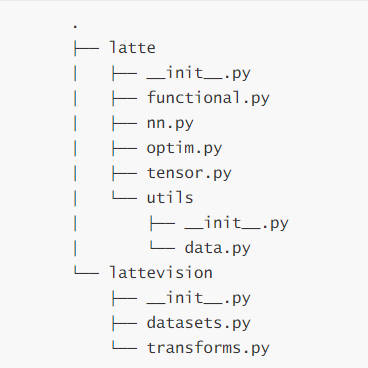
\includegraphics[width=0.4\textwidth]{./img/tree.jpg}
	\caption{Package Structure}
\end{figure}

Latte packages some basic modules, like \textbf{tensor} defines the basic data structure,
\textbf{nn} together with \textbf{functional} provides necessary classes and functions
for neural network, \textbf{optim} includes some classical optimization methods, and
\textbf{utils.data} is for dataset and data loader. All the interfaces are referred to
the official documentation of PyTorch.

Furthermore, what torchvision is to torch, lattevision is to latte. It includes some
requisite modules for computer vision tasks. To be more specific, \textbf{transforms}
contains some transformation functions for image processing, \textbf{datasets} implements
the downloading and loading of MNIST dataset for now.

All the features above are implemented using \textbf{numpy} package.

For more information, please refer to the source code.

\subsection{\textbf{Module tensor}}

Tensor is the basic data structure in Latte which wraps the \textbf{numpy array} together
with some other features such as \textbf{gradient}, \textbf{require grad}, and so on.

One important feature need to be noted is that tensor basically reproduces
\textbf{Computational Graph} for every single operation in matrix computation.

\subsection{\textbf{Module nn \& functional}}

These two modules are the core of the framework. They are used to define the neural network
layers like \textbf{Linear}, \textbf{Sigmoid}, \textbf{ReLU}, \textbf{Dropout} and loss
functions like \textbf{MSELoss}, \textbf{BCELoss}, \textbf{CrossEntropyLoss}.

\subsection{\textbf{Module optim}}

Manually implementation of \textbf{SGD} and \textbf{Adam}.

Also the \textbf{L2 regularization} is provided as the interface of \textbf{weight decay}.

\subsection{\textbf{Quick Start}}

This part is a quick start guide, we run a toy example to see whether the framework works. By
the way, all the code implementations are included in \textbf{quick start} jupyter notebooks.

As an example, we use only \textbf{fully connected} layers to build a simple network, the
activation function is \textbf{ReLU}. For criterion and optimizer, we simply use
\textbf{CrossEntropyLoss} and \textbf{Adam} respectively.

The nerwork architecture is shown in the following figure:

\begin{figure}[H]
	\centering
	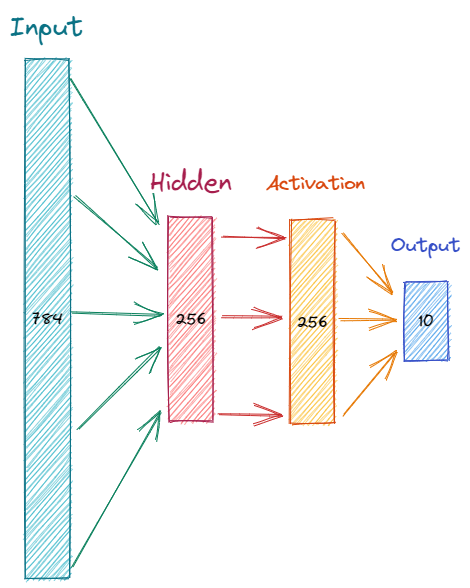
\includegraphics[width=0.42\textwidth]{./img/simple-network.png}
	\caption{Simple Network}
\end{figure}

Finally we get the accuracy \textbf{96.59\%}. In the next part, we will do some search on
hyperparameters to find the best model.

\bigskip

%------------------------------------------------

\section{\textbf{Hyperparameter Search}}

Instead of making attempts in different learning rate, we apply a \textbf{decreasing scheme}
for learning rate. The learning rate is set to \textbf{0.01} initially, and we decrease it
by a factor of \textbf{0.9} when the validation loss does not improve.

Then we search for the best \textbf{hidden units} and \textbf{weight decay} in the space of
\textbf{[64, 128, 256, 512]} and \textbf{[0, 1e-5]} respectively.

Here's the result:

\begin{table}[H]
	\begin{center}
		\begin{tabular}{ccccc}
			\toprule
			Units & Weight Decay & Best Val Loss & Best Val Acc & Test Acc         \\
			\midrule
			64    & 0            & 0.0055        & 95.56\%      & 96.50\%          \\
			64    & 1e-5         & 0.0050        & 96.24\%      & 96.44\%          \\
			128   & 0            & 0.0047        & 96.60\%      & 97.22\%          \\
			128   & 1e-5         & 0.0044        & 96.68\%      & 97.23\%          \\
			256   & 0            & 0.0042        & 96.83\%      & 97.47\%          \\
			256   & 1e-5         & 0.0039        & 97.43\%      & 97.61\%          \\
			512   & 0            & 0.0041        & 97.36\%      & 97.85\%          \\
			512   & 1e-5         & 0.0039        & 97.38\%      & \textbf{97.92\%} \\
			\bottomrule
		\end{tabular}
		\caption{Number of Hidden Units}
	\end{center}
\end{table}

And the training process for the best model is shown in the following figure:

\begin{figure}[H]
	\centering
	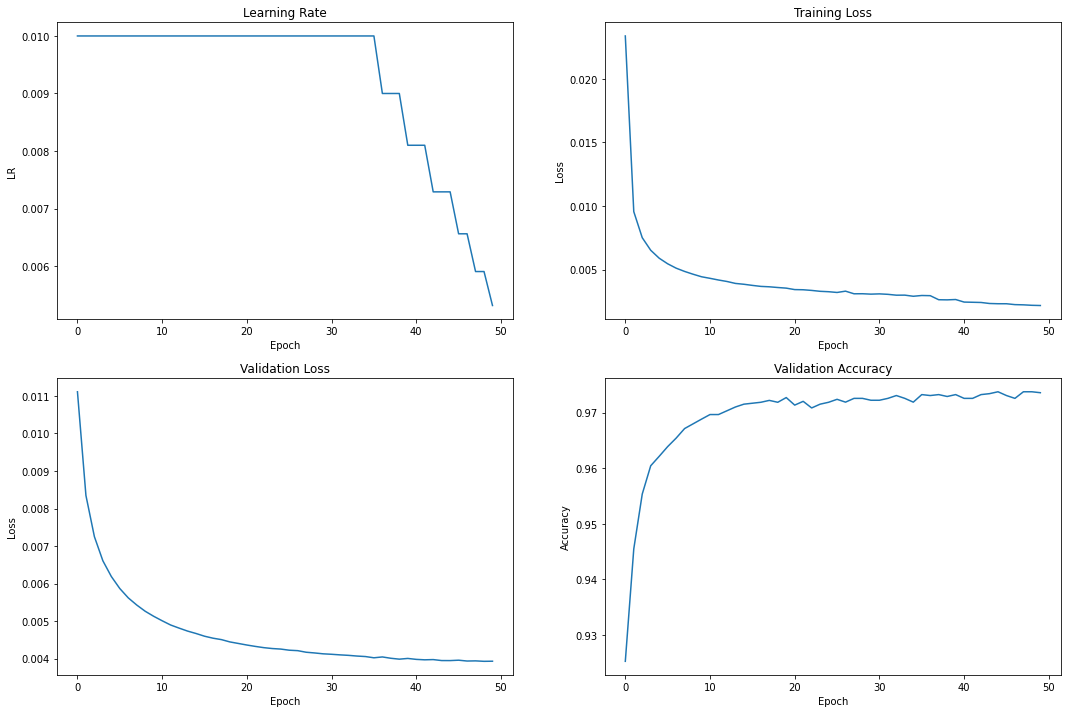
\includegraphics[width=0.9\textwidth]{./img/train-process.png}
	\caption{Training Process}
\end{figure}

More details for other models can be found in the \textbf{hyperparam search} jupyter notebook.

\bigskip

%------------------------------------------------

\section{\textbf{Parameter Visualization}}

The visualization of the best model's parameters in heatmap is as follows:

\begin{figure}[H]
	\centering
	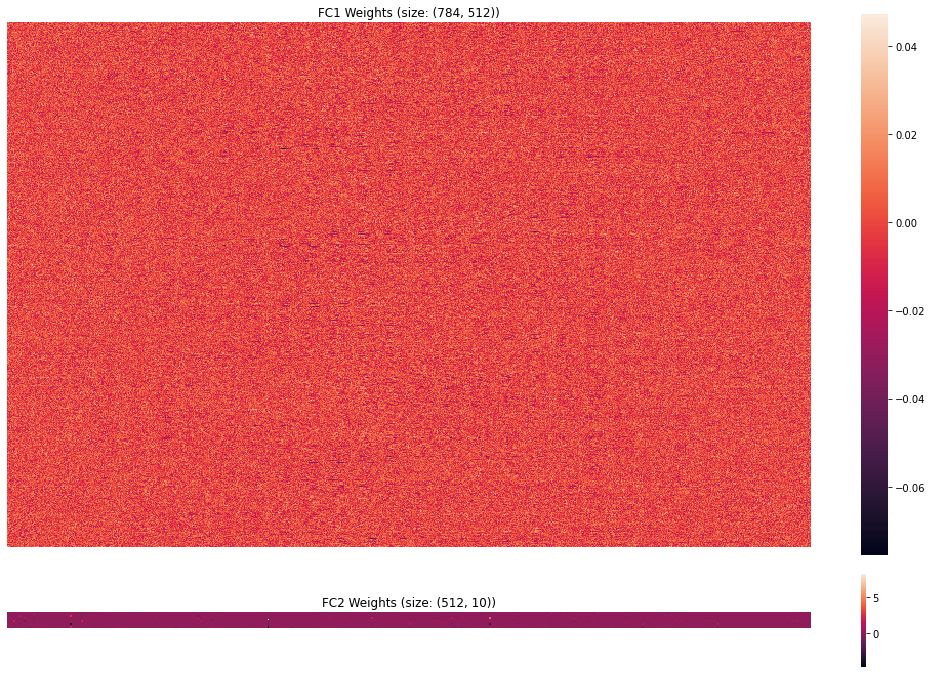
\includegraphics[width=0.9\textwidth]{./img/heatmap-512.png}
	\caption{Heatmap Best}
\end{figure}

\begin{figure}[H]
	\centering
	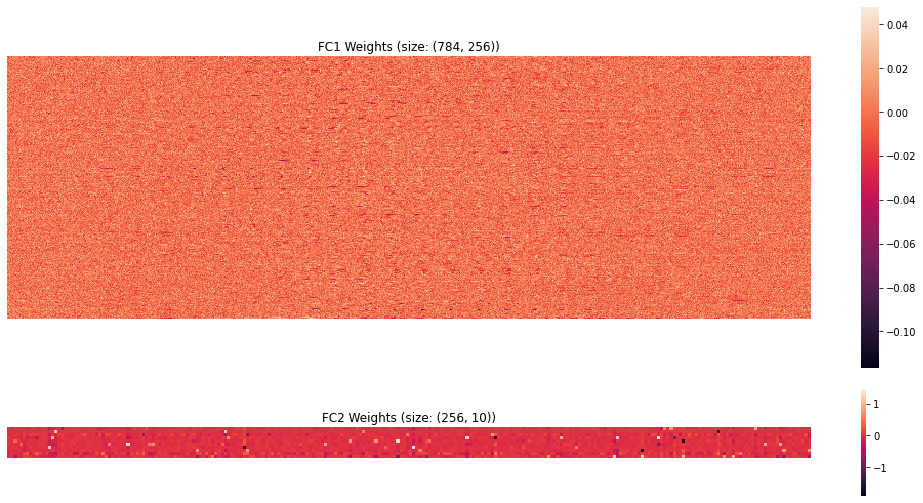
\includegraphics[width=0.9\textwidth]{./img/heatmap-256.png}
	\caption{Heatmap 256}
\end{figure}

We can find some implicit grids in the heatmap regularly.

\bigskip

%----------------------------------------------------------------------------------------
%	REFERENCE LIST
%----------------------------------------------------------------------------------------

% \cite{Eureka}
% \printbibliography

%----------------------------------------------------------------------------------------

\end{document}
